\documentclass[letterpaper]{article} % DO NOT CHANGE THIS
\usepackage{aaai2027}  % DO NOT CHANGE THIS
% Serif, sans-serif, and monospaced fonts are loaded automatically by
% aaai2027.sty (T1 fontenc, newtxtext, helvet, courier).
% DO NOT add times, helvet, courier, geometry, hyperref, or other disallowed packages.
\usepackage[hyphens]{url}  % DO NOT CHANGE THIS
\usepackage{graphicx} % DO NOT CHANGE THIS
\urlstyle{rm} % DO NOT CHANGE THIS
\def\UrlFont{\rm}  % DO NOT CHANGE THIS
\usepackage{natbib}  % DO NOT CHANGE THIS AND DO NOT ADD ANY OPTIONS TO IT
\usepackage{caption} % DO NOT CHANGE THIS AND DO NOT ADD ANY OPTIONS TO IT
\frenchspacing  % DO NOT CHANGE THIS

% Suporte a português (hifenização, rótulos Figura/Tabela/Resumo) e matemática/tabelas
\usepackage[brazilian]{babel}
\usepackage{amsmath}
\usepackage{booktabs}

\pdfinfo{
/TemplateVersion (2027.2)
}

\setcounter{secnumdepth}{1}

\title{Classificação de Dígitos Manuscritos com Rede Neural Artificial de Duas Camadas no Conjunto MNIST}
\author{
    Rafael Sant'Ana
}
\affiliations{
    Departamento de Ciência da Computação (DCC) --- Universidade Federal de Minas Gerais (UFMG)\\
    DCC642 --- Introdução à Inteligência Artificial (2026/2)\\
    rafael.santana@dcc.ufmg.br
}

\begin{document}

\maketitle

\begin{abstract}
Este trabalho aborda o reconhecimento de dígitos manuscritos no MNIST (70.000 imagens $28 \times 28$, 10 classes) por meio de um MLP de duas camadas ($784 \to h \to 10$) em NumPy (\texttt{learn.py}), com ativação ReLU, saída Softmax numericamente estável, perda de entropia cruzada e treinamento via gradiente descendente em lote completo (\emph{full-batch GD}). A partir da base ($\alpha = 0{,}1$, 200 épocas, $h = 64$), variaram-se controladamente a taxa de aprendizado ($\alpha \in \{0{,}001;\; 0{,}01;\; 0{,}1;\; 0{,}5\}$), as épocas ($\{50;\; 100;\; 200;\; 500\}$) e os neurônios escondidos ($h \in \{4;\; 16;\; 64;\; 256\}$). O melhor modelo ($\alpha = 0{,}5$, 200 épocas, $h = 64$) atingiu 92,43\% de acurácia de teste (perda de treino $0{,}2585$), superando o limiar de 90\%. Os resultados evidenciam forte sensibilidade à taxa de aprendizado e compromissos entre capacidade, tempo de treino e generalização.

\end{abstract}

\section{Introdução e Objetivo}

O reconhecimento automático de dígitos manuscritos (de 0 a 9) é um problema clássico de visão computacional e aprendizado de máquina, amplamente utilizado para validar modelos de classificação multiclasse. Nesse cenário, o conjunto de dados MNIST consolida-se como referência padrão, reunindo 70.000 imagens em escala de cinza com resolução de $28 \times 28$ pixels. Quando vetorizada, cada imagem corresponde a um vetor de 784 atributos numéricos, permitindo que modelos conexionistas aprendam fronteiras de decisão não lineares diretamente a partir das intensidades de pixel, sem extração manual de características.

O objetivo deste trabalho é implementar do zero, em Python com NumPy (\texttt{learn.py}), uma Rede Neural Artificial do tipo Perceptron Multicamadas (MLP) de duas camadas, composta por uma camada escondida com ativação ReLU e uma camada de saída com função Softmax. Especificamente, busca-se: (i)~implementar a inicialização de parâmetros, as funções de ativação, a propagação direta, a perda de entropia cruzada, a atualização por gradiente descendente e a métrica de acurácia; (ii)~avaliar sistematicamente o impacto da taxa de aprendizado, do número de épocas e da largura da camada escondida sobre a perda de treinamento, a acurácia de teste e o tempo computacional; e (iii)~obter uma configuração com acurácia de teste $\ge 90\%$, validando qualitativamente seu comportamento na interface interativa de desenho (\texttt{server.py}).

\section{Metodologia}

\noindent\textbf{Conjunto de Dados e Pré-processamento.}
Utilizamos o conjunto de dados \texttt{mnist\_784}, obtido via \texttt{fetch\_openml}, composto por $70.000$ imagens de dígitos manuscritos ($28 \times 28$ pixels) vetorizadas em $784$ atributos. As intensidades de pixel, originalmente no intervalo $[0, 255]$, são normalizadas para $[0, 1]$ mediante divisão por $255{,}0$. Os dados são particionados na proporção 80/20 (\texttt{test\_size=0.2}, \texttt{random\_state=42}), resultando em $m = 56.000$ exemplos de treinamento e $14.000$ de teste. Os rótulos das $C = 10$ classes são convertidos para a representação \emph{one-hot} com \texttt{OneHotEncoder}, ajustado no conjunto de treino e aplicado ao de teste. Toda a lógica da rede neural e de otimização é implementada diretamente em NumPy.

\noindent\textbf{Arquitetura e Inicialização.}
Adotamos uma rede neural \emph{feedforward} totalmente conectada (MLP) de duas camadas ($784 \to h \to 10$), onde $h$ representa o número de neurônios na camada escondida (\texttt{hidden\_size}). As matrizes de pesos $W_1$, de dimensão $784 \times h$, e $W_2$, de dimensão $h \times 10$, são inicializadas a partir de $\mathcal{N}(0, 0{,}01^2)$ (\texttt{np.random.randn * 0.01}) sob semente global fixa (\texttt{np.random.seed(42)}), quebrando a simetria entre neurônios sem saturar as ativações iniciais. Os vetores de viés $b_1$ ($1 \times h$) e $b_2$ ($1 \times 10$) são inicializados com zeros.

\noindent\textbf{Propagação Direta e Ativações.}
Dado um lote de entradas $X$, a propagação direta (\emph{forward pass}) computa as pré-ativações e ativações das camadas escondida e de saída segundo:
\begin{gather*}
Z_1 = X W_1 + b_1, \quad A_1 = \text{ReLU}(Z_1) = \max(0, Z_1), \\
Z_2 = A_1 W_2 + b_2, \quad A_2 = \text{softmax}(Z_2).
\end{gather*}
Na função \emph{softmax}, para assegurar estabilidade numérica, subtrai-se o valor máximo por amostra ($z_j - \max_k z_k$) antes da exponenciação, mantendo os argumentos não positivos e prevenindo \emph{overflow} numérico sem alterar a distribuição de probabilidades resultante.

\noindent\textbf{Função de Perda, Otimização e Avaliação.}
O treinamento minimiza a entropia cruzada multiclasse:
\[
L = -\frac{1}{m}\sum_{i=1}^{m}\sum_{c=1}^{C} y_{ic}\log(\hat{y}_{ic}),
\]
com \emph{clipping} das probabilidades preditas $\hat{y}_{ic}$ no intervalo $[10^{-12}, 1{,}0]$ antes do logaritmo para evitar $\log(0)$ e valores indefinidos. O ajuste dos parâmetros utiliza gradiente descendente em lote completo (\emph{full-batch GD}): a cada época, calculam-se os gradientes exatos por retropropagação (\texttt{backward}) sobre todos os $m = 56.000$ exemplos, empregando $dZ_2 = A_2 - Y$ na saída, $\text{ReLU}'(Z_1) = \mathbf{1}[Z_1 > 0]$ na camada escondida e normalização por $m$, atualizando cada parâmetro via $\theta \leftarrow \theta - \alpha \nabla_\theta L$. O desempenho é medido pela acurácia no conjunto de teste, comparando os índices de maior probabilidade (\texttt{argmax}) entre as saídas preditas e os rótulos \emph{one-hot}.

\noindent\textbf{Protocolo Experimental.}
Realizamos uma varredura controlada variando apenas um hiperparâmetro por vez a partir da configuração-base fixa ($\alpha = 0{,}1$, $200$ épocas e $h = 64$ neurônios escondidos, com semente \texttt{42}), totalizando dez configurações distintas nos eixos $\alpha \in \{0{,}001;\, 0{,}01;\, 0{,}1;\, 0{,}5\}$, épocas em $\{50, 100, 200, 500\}$ e $h \in \{4, 16, 64, 256\}$. Em cada execução, sob a mesma divisão treino/teste, registram-se a perda final de treinamento, a acurácia final de teste e o tempo total de execução em CPU.

\section{Experimentos e Resultados}

Para avaliar o impacto dos hiperparâmetros no desempenho da MLP treinada com gradiente descendente em lote completo sobre o conjunto MNIST, executou-se uma varredura univariada a partir da configuração de referência ($\alpha = 0{,}1$, $200$ épocas, $h = 64$ neurônios e semente $42$), resumida na Tabela~\ref{tab:experimentos}. Observa-se que a taxa de aprendizado exerce o efeito mais acentuado: valores reduzidos ($\alpha \in \{0{,}001; 0{,}01\}$) praticamente impedem a convergência em $200$ épocas, enquanto $\alpha = 0{,}5$ reduz a perda para $0{,}2585$ e eleva a acurácia de teste para $92{,}43\%$ em apenas $280{,}6$~s. O aumento do número de épocas promove ganhos consistentes com crescimento quase linear do tempo de execução, atingindo $90{,}21\%$ em $500$ épocas ($729{,}3$~s). Já a expansão da camada escondida apresenta retornos decrescentes: de $h = 4$ para $h = 256$, a acurácia sobe de $69{,}26\%$ para $87{,}63\%$, mas o custo computacional cresce mais de dez vezes ($922{,}4$~s).

\begin{table}[t]
\centering
\small
\setlength{\tabcolsep}{4pt}
\begin{tabular}{lrrrr}
\toprule
Grupo & Valor & Perda & Acurácia (\%) & Tempo (s) \\
\midrule
Taxa ($\alpha$) & 0,001 & 2,3016 & 12,71 & 353,5 \\
                & 0,01 & 2,2840 & 30,61 & 355,7 \\
                & 0,1$^\dagger$ & 0,5320 & 86,11 & 355,5 \\
                & \textbf{0,5} & \textbf{0,2585} & \textbf{92,43} & \textbf{280,6} \\
\midrule
Épocas          & 50 & 2,1144 & 44,28 & 113,9 \\
                & 100 & 1,0912 & 76,28 & 196,4 \\
                & 200$^\dagger$ & 0,5320 & 86,11 & 355,5 \\
                & \textbf{500} & \textbf{0,3417} & \textbf{90,21} & \textbf{729,3} \\
\midrule
Escondida ($h$) & 4 & 0,9421 & 69,26 & 84,7 \\
                & 16 & 0,6374 & 83,74 & 115,9 \\
                & 64$^\dagger$ & 0,5320 & 86,11 & 355,5 \\
                & \textbf{256} & \textbf{0,4755} & \textbf{87,63} & \textbf{922,4} \\
\bottomrule
\end{tabular}
\caption{Resultados da varredura de hiperparâmetros no conjunto de teste MNIST. O símbolo $^\dagger$ marca a configuração de referência ($\alpha = 0{,}1$, $200$ épocas, $h = 64$, semente $42$), e o negrito destaca o melhor resultado de cada bloco.}
\label{tab:experimentos}
\end{table}

Duas configurações da varredura superaram a meta de $90\%$ de acurácia no teste: $500$ épocas ($90{,}21\%$ em $729{,}3$~s) e $\alpha = 0{,}5$ ($92{,}43\%$ em $280{,}6$~s), sendo esta última superior tanto em precisão quanto em eficiência. A Figura~\ref{fig:curvas} ilustra a evolução da perda de entropia cruzada e da acurácia ao longo das $200$ épocas para os quatro valores de $\alpha$. Com $\alpha = 0{,}5$, a perda cai abruptamente nas iterações iniciais e a acurácia cresce de forma acelerada até atingir $92{,}43\%$. A referência ($\alpha = 0{,}1$) apresenta queda moderada e contínua, ao passo que $\alpha = 0{,}01$ progride lentamente e $\alpha = 0{,}001$ permanece quase estagnado próximo à perda inicial de um classificador uniforme ($\ln 10 \approx 2{,}3026$).

% [TODO: se houver melhor modelo dedicado >=90% finalizado, atualizar figura e métricas]
\begin{figure}[t]
\centering
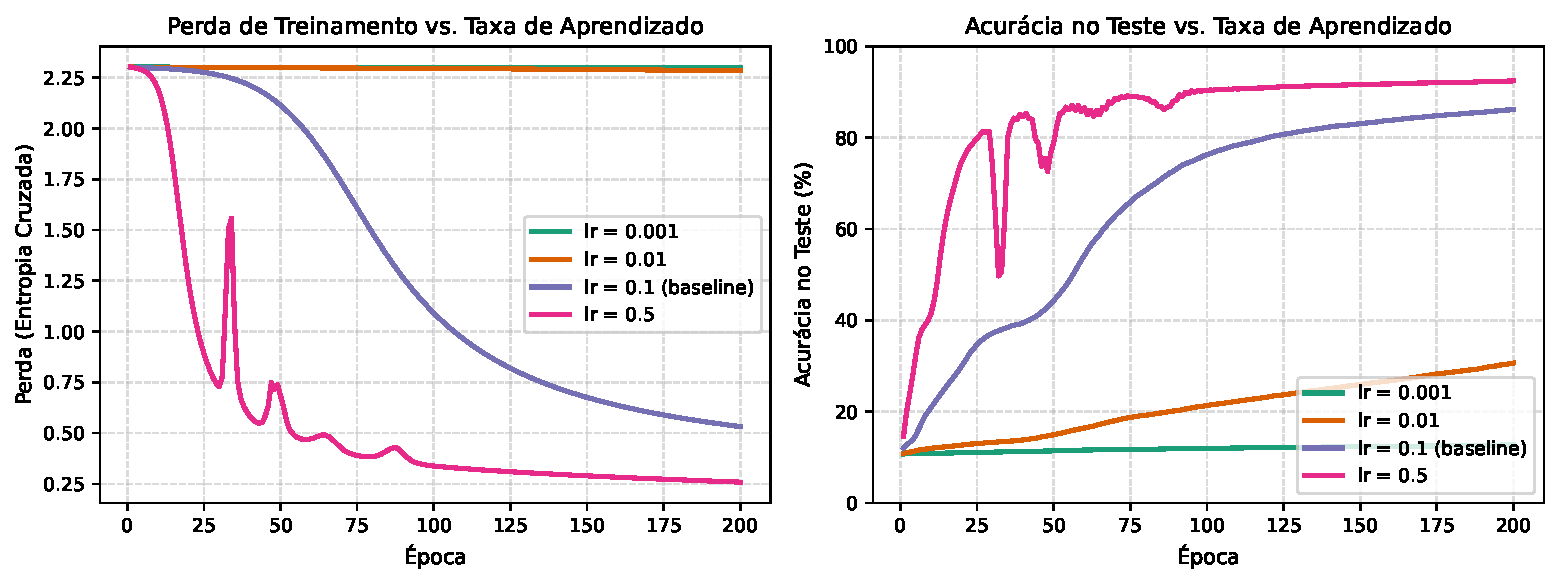
\includegraphics[width=\columnwidth]{figures/sweep_learning_rate.pdf}
\caption{Curvas de perda e acurácia ao longo de $200$ épocas para $\alpha \in \{0{,}001; 0{,}01; 0{,}1; 0{,}5\}$ com $h = 64$, destacando a convergência da melhor configuração ($\alpha = 0{,}5$, $92{,}43\%$).}
\label{fig:curvas}
\end{figure}

\subsection{Análise Qualitativa na Interface Interativa}

Para complementar a avaliação quantitativa, carregaram-se os pesos do melhor modelo ($\ge 90\%$ de acurácia) na interface web de \texttt{server.py} (\texttt{http://localhost:5001}), desenhando-se dígitos manuscritos na grade $28 \times 28$. Nos testes interativos, [TODO: preencher com os 3+ dígitos desenhados na interface, indicando a classe predita e a confiança Softmax obtida em cada caso]. Quanto aos padrões de acerto e erro, [TODO: preencher com os 3+ dígitos desenhados na interface --- quais dígitos foram reconhecidos com maior confiabilidade e quais pares sofreram confusão]. Esse comportamento reflete propriedades estruturais da MLP: como cada pixel de entrada possui pesos independentes, a predição depende fortemente da espessura do traço e da centralização na grade $28 \times 28$, evidenciando a sensibilidade da rede totalmente conectada a pequenas translações em relação ao padrão do MNIST.

\section{Discussão}

\textbf{Convergência versus estabilidade.} A taxa de aprendizado $\alpha$ mostrou-se o hiperparâmetro mais determinante. Com $\alpha = 0{,}001$, a perda estagnou em $2{,}3016$ --- próxima à entropia uniforme $\ln(10) \approx 2{,}3026$ --- com acurácia de $12{,}71\%$ (nível do acaso); já $\alpha = 0{,}01$ atingiu apenas $30{,}61\%$ (perda $2{,}2840$). Como o \textit{full-batch} executa uma única atualização por época e os pesos iniciais são pequenos ($\sigma = 0{,}01$), os gradientes iniciais têm baixa magnitude e $200$ passos são insuficientes. Elevar $\alpha$ para $0{,}1$ e $0{,}5$ acelerou fortemente a convergência, atingindo $86{,}11\%$ (perda $0{,}5320$) e $92{,}43\%$ (perda $0{,}2585$, em $280{,}6$~s), embora taxas excessivas induzissem oscilações ou divergência.

\textbf{Retornos decrescentes e orçamento computacional.} Variar o número de épocas (com $\alpha = 0{,}1$ e $h = 64$) evidencia ganhos marginais decrescentes. Dobrar de $50$ para $100$ épocas reduziu a perda de $2{,}1144$ para $1{,}0912$ e elevou a acurácia em $+32{,}00$ pontos percentuais (p.p.), de $44{,}28\%$ ($113{,}9$~s) para $76{,}28\%$ ($196{,}4$~s). De $100$ para $200$ épocas, o ganho caiu para $+9{,}83$~p.p. ($86{,}11\%$, $355{,}5$~s). Adicionar mais $300$ épocas ($200 \to 500$) rendeu apenas $+4{,}10$~p.p. ($90{,}21\%$, perda $0{,}3417$), mais que dobrando o tempo ($355{,}5$~s $\to$ $729{,}3$~s).

\textbf{Capacidade da rede versus custo e generalização.} Com $h = 4$ ($3.190$ parâmetros), ocorre claro \textit{underfitting} ($69{,}26\%$, perda $0{,}9421$, $84{,}7$~s) pelo gargalo informacional para $10$ classes. Como os parâmetros escalam linearmente ($784h + h + 10h + 10$), expandir $h$ para $16$, $64$ e $256$ eleva o total para $12.730$, $50.890$ e $203.530$ parâmetros e o tempo de $115{,}9$~s para $355{,}5$~s e $922{,}4$~s. Apesar do avanço até $h = 64$ ($83{,}74\% \to 86{,}11\%$), quadruplicar para $h = 256$ adicionou apenas $+1{,}52$~p.p. ($87{,}63\%$, perda $0{,}4755$), elevando o risco de \textit{overfitting} sob treinos mais longos.

\textbf{Limitações arquiteturais e algorítmicas.} Três fatores restringem o modelo atual: (i) o \textit{full-batch GD} atualiza os pesos apenas uma vez a cada $56.000$ exemplos; (ii) a inicialização gaussiana fixa ($\sigma = 0{,}01$) não escala com o \textit{fan-in}, diferentemente da inicialização de He para ReLU; e (iii) o achatamento de imagens $28 \times 28$ em vetores de $784$ dimensões descarta a topologia espacial 2D, tornando o MLP sensível a translações, rotações e variações de espessura de traço em entradas desenhadas à mão.

\section{Conclusão}

Neste trabalho, implementou-se com sucesso, do zero em NumPy, um Perceptron Multicamadas de duas camadas ($784 \to h \to 10$) para classificação de dígitos manuscritos do conjunto MNIST. A melhor configuração obtida ($\alpha = 0{,}5$, 200 épocas e $h = 64$) alcançou \textbf{92,43\%} de acurácia no conjunto de teste, com perda final de $0{,}2585$ em $280{,}6$~s, superando o critério mínimo de 90\%. Os experimentos evidenciaram a elevada sensibilidade aos hiperparâmetros --- especialmente à taxa de aprendizado no \textit{full-batch GD} ---, bem como o compromisso entre capacidade representacional e custo computacional.

Como trabalhos futuros, quatro aprimoramentos são particularmente promissores: (i)~substituir o gradiente em lote completo por \textit{mini-batch SGD} com \textit{momentum} ou \textbf{Adam}, acelerando substancialmente a convergência; (ii)~adotar a \textbf{inicialização de He} ($\mathcal{N}(0, 2/n_{\text{in}})$), mais adequada à ativação ReLU para preservar a variância dos gradientes; (iii)~incorporar regularização $L_2$, \textit{Dropout} e \textit{data augmentation} (pequenas translações e rotações) para ampliar a generalização; e (iv)~explorar \textbf{Redes Neurais Convolucionais (CNNs)}, que preservam a estrutura espacial 2D das imagens e conferem invariância a translações.

\section*{Declaração de Uso de IA}

Declara-se o uso de ferramentas de IA generativa (assistente de código) como apoio na configuração do template \LaTeX{} AAAI-27, no desenvolvimento de scripts auxiliares para automação dos experimentos, coleta de métricas e geração de gráficos, bem como na revisão estrutural e redacional deste relatório. A implementação central da rede neural (\texttt{learn.py}), a validação experimental dos resultados e a análise crítica foram integralmente revisadas e validadas pelo autor. Os registros das conversas estão disponíveis em: [TODO: inserir links das conversas realizadas].


\end{document}
